\documentclass[tikz,border=6pt]{standalone}
\usepackage{amsmath}
\usepackage{xcolor}

\definecolor{blockblue}{HTML}{4A90D9}

\begin{document}
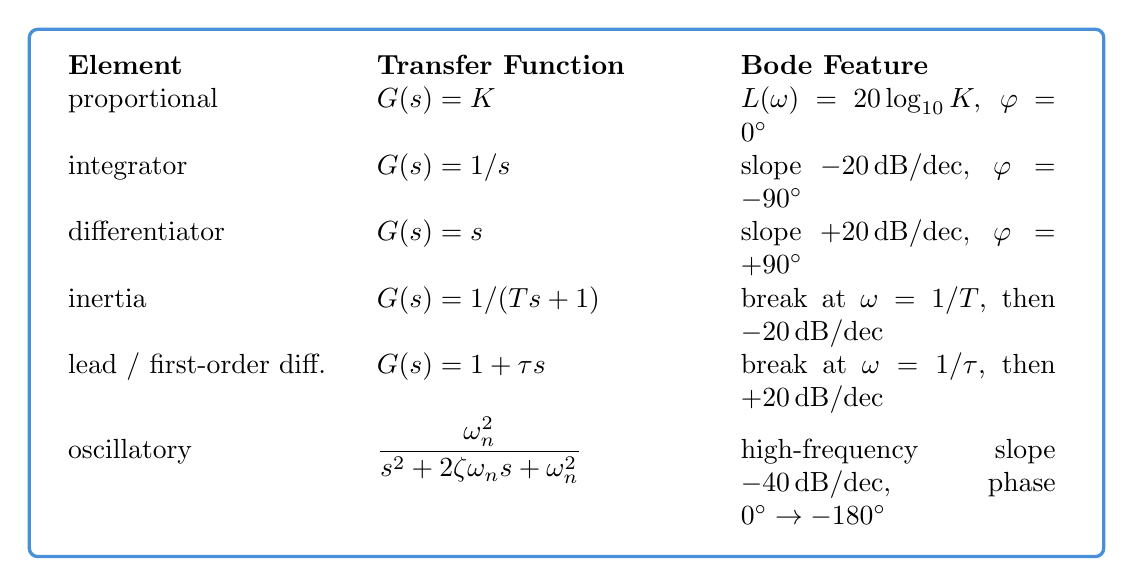
\begin{tikzpicture}[line width=1.2pt]
  \node[
    draw=blockblue,
    rounded corners=3pt,
    inner sep=8pt,
    align=left
  ] at (0,0) {
    \begin{tabular}{p{3.5cm}p{4.2cm}p{4.0cm}}
      \textbf{Element} & \textbf{Transfer Function} & \textbf{Bode Feature} \\
      proportional & $G(s)=K$ & $L(\omega)=20\log_{10}K,\ \varphi=0^\circ$ \\
      integrator & $G(s)=1/s$ & slope $-20\,\mathrm{dB/dec},\ \varphi=-90^\circ$ \\
      differentiator & $G(s)=s$ & slope $+20\,\mathrm{dB/dec},\ \varphi=+90^\circ$ \\
      inertia & $G(s)=1/(Ts+1)$ & break at $\omega=1/T$, then $-20\,\mathrm{dB/dec}$ \\
      lead / first-order diff. & $G(s)=1+\tau s$ & break at $\omega=1/\tau$, then $+20\,\mathrm{dB/dec}$ \\
      oscillatory & $\dfrac{\omega_n^2}{s^2+2\zeta\omega_n s+\omega_n^2}$ & high-frequency slope $-40\,\mathrm{dB/dec}$, phase $0^\circ \to -180^\circ$ \\
    \end{tabular}
  };
\end{tikzpicture}
\end{document}
